% !TEX program = xelatex
% -------------------------------------------------------
\documentclass[nols, a4paper]{tufte-handout}

% --- 基础设置与宏包 ---
\usepackage{graphicx}
\usepackage{booktabs}
\usepackage{amsmath}
\usepackage{lipsum}
\usepackage{hyperref}
\hypersetup{colorlinks, allcolors=blue}

% 设置全文行距为 1.5 倍 ---
\usepackage{setspace}

% 自定义标题样式并强制编号 ---
\usepackage{titlesec}

% 设置代码块格式
\usepackage{listings}
\lstset{
 columns=fixed,       
 numbers=none,                                        % 在左侧显示行号
 numberstyle=\tiny\color{gray},                       % 设定行号格式
 frame=none,                                          % 不显示背景边框
 backgroundcolor=\color[RGB]{245,245,244},            % 设定背景颜色
 keywordstyle=\color[RGB]{40,40,255},                 % 设定关键字颜色
 numberstyle=\footnotesize\color{darkgray},           
 commentstyle=\it\color[RGB]{0,96,96},                % 设置代码注释的格式
 stringstyle=\rmfamily\slshape\color[RGB]{128,0,0},   % 设置字符串格式
 showstringspaces=false,                              % 不显示字符串中的空格
 language=python,                                        % 设置语言
}

% 设置编号深度
\setcounter{secnumdepth}{3} 

% 格式化一级标题 ,在标题后加横线
\titleformat{\section}[display]
  {\normalfont\Large\bfseries}
  {\thesection}
  {1em}
  {}
  [\vspace{1ex}\hrule]

% 格式化二级标题
\titleformat{\subsection}
  {\normalfont\large\bfseries}
  {\thesubsection} % <-- 加入编号
  {1em}
  {}

% 格式化三级标题 (paragraph)
\renewcommand{\theparagraph}{\thesubsection.\arabic{paragraph}}
\titleformat{\paragraph}
  {\normalfont\normalsize\bfseries}
  {\theparagraph} % <-- 加入编号
  {1em}
  {}

% 字体设置 
\usepackage{xeCJK}
\setmainfont{Times New Roman}
\setsansfont{Arial} 
\setmonofont{Courier New}
\setCJKmainfont{STFangsong}
\setCJKsansfont{STHeiti}
\setCJKmonofont{STFangsong}

% 解决图表标题的中文问题
\usepackage{caption}
% 全局设置:表格标题在上方,图片标题在下方。
\captionsetup[table]{position=top}
\captionsetup[figure]{position=bottom}
\captionsetup{font=small, labelfont=bf}
\usepackage{subcaption}

% ----------------------------------------------------------------------
% 页面布局调整 (核心部分)
% ----------------------------------------------------------------------
\usepackage{geometry}
\geometry{
  a4paper,
  left=20mm,
  top=35mm, 
  bottom=25mm,
  textwidth=113mm,
  marginparwidth=51mm,
  marginparsep=5mm
}

% --- 文档信息 ---
\title{Neuron modeling discussion}
\author{独宇涵}
\date{\today}

\begin{document}

% 应用 1.5 倍行距
\onehalfspacing 

\maketitle

\tableofcontents

% --- 优化 2: 在目录后添加分界线 ---
\bigskip
\noindent\rule{\linewidth}{0.4pt}
\bigskip

\section{LIF model(Integrate and Fire)}

\subsection{模型概述} 

LIF模型只考虑神经细胞膜的被动特性以及动作电位的触发,即将模型简化为电容、电池以及可变电阻的并联,再在此基础上并联一个外部电流输入(如图 \ref{LIF})

\begin{marginfigure}
  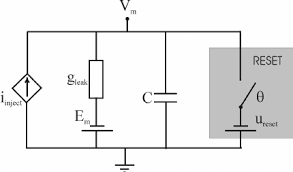
\includegraphics[width=\linewidth]{image/LIF.png} 
  % 图片的标题在下方,是正确的
  \caption{图片来自\href{https://www.researchgate.net/figure/Simplied-circuit-of-the-LIF-neuron-model_fig1_232262611}{Google}}
  \label{LIF}
\end{marginfigure}

该模型的工作原理可以采用下面的公式来表示,公式表现出了膜电位的工作特性以及外部电流$I_\text{inj}$对膜电位的影响。

\[
C_m \frac{dV}{dt} = -g_L (V - E_L) + I_\text{inj}
\]

其中$C_m$代表细胞膜表面的电容,$g_L$表示细胞膜的漏电导,$E_L$表示漏电平衡电压(决定了细胞膜在无信号输入时的平衡点)。整个微分方程满足基尔霍夫定律,即流入节点的电流等于流出的电流。
除此之外,在电位超过给定阈值($V_{th}$)后就会产生一个Spike并且将膜电位重置到一个重置电位($V_{reset}$),之后则会维持一个不应期(Refractory period:$tau_{ref}$),处于不应期时细胞膜电位并不会对外在刺激做出反应

根据上述方程以及LIF模型的工作原理,很容易补全代码的空余部分,在初始设置下(C\_m = 1.0,g\_L = 0.1,E\_L = -70.0
V\_th = -55.0,V\_reset = -75.0,V\_spike = 20,tau\_ref = 2.0)运行得到的结果如图\ref{LIF_default}所示

\begin{figure*}
  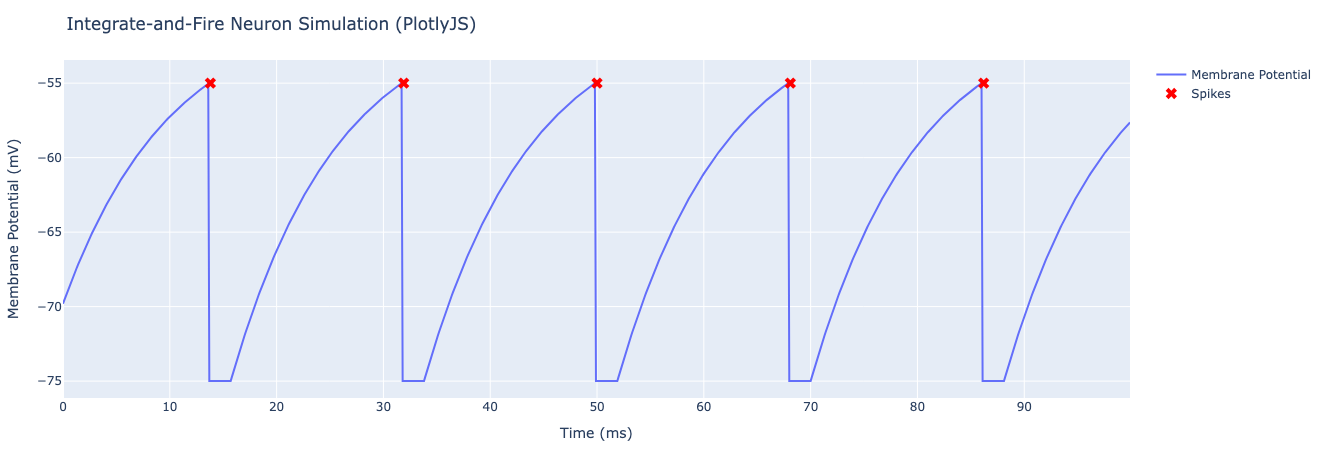
\includegraphics[width=\linewidth]{image/LIF_default.png} 
  % 图片的标题在下方,是正确的
  \caption{初始设置下运行的结果}
  \label{LIF_default}
\end{figure*}


\subsection{改变$g_L$、$C_m$、$I_{inj}$}

首先来研究$g_L$和输入电流$I_{inj}$对模型的影响。
从微分方程中不难看出,存在稳态电位$V_{\inf} = E_L + \frac{I_{inj}}{g_L}$,在固定$E_L$的前提下,输入电流越大则稳态时电压越高,而$g_L$越大稳态时电压越小,甚至有可能无法达到阈值$V_{th}$而无法产生spike。
对于$I_{inj} = 2$的情况我们可以计算出产生spike时$g_L$需要满足:$g_L < \frac{2}{15}$,
\begin{marginfigure}
  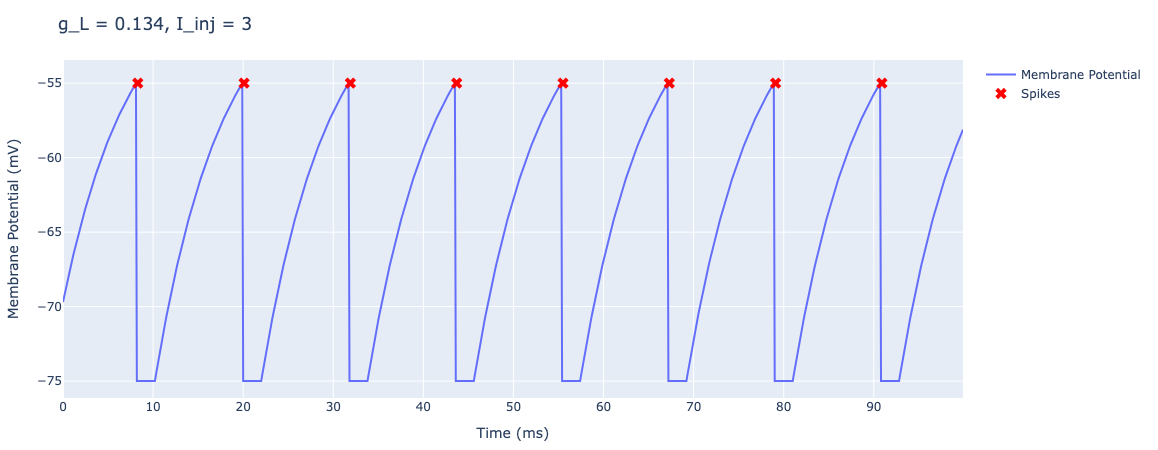
\includegraphics[width=\linewidth]{image/g0134i3.png} 
  % 图片的标题在下方,是正确的
  \caption{g\_L = 0.134, I\_inj = 3}
  \label{g0.134I3}
\end{marginfigure}
当小于这个数值可以产生spike,如果大于这个数值则无法产生spike (如图\ref{g0.134I2}),此时如果增大输入电流的值则可以重新产生spike(如图\ref{g0.134I3})

\begin{figure*}
  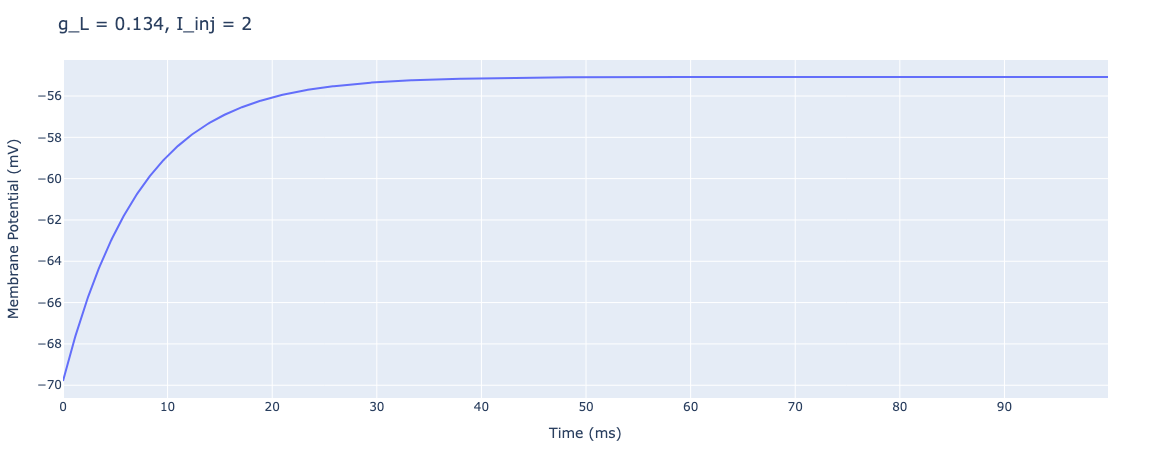
\includegraphics[width = 0.94\linewidth]{image/g0134i2.png} 
  % 图片的标题在下方,是正确的
  \caption{g\_L = 0.134, I\_inj = 2}
  \label{g0.134I2}
\end{figure*}

当讨论$C_m$对模型的影响时,我们从上面的公式中不难看出,膜电容大小虽然不会对稳态电位产生影响,但是却影响达到稳态电位所需要的时间。
在搜集一些资料后找到一个很有趣的概念——膜时间常数(tau),在LIF模型下可以表示为$tau = \frac{C_m}{g_L}$。

在输入电流为$I_{inj} = 2$的前提下,不同$g_L$和$C_m$下的模型产生spike到恢复的间隔统计结果汇总在下表\ref{g_L}之中

\begin{table}[h!]
    % 这个表格的标题位置本来就是正确的
    \caption{不同$g_L$和$C_m$下的间隔}
    \label{g_L}
    \begin{tabular*}{\textwidth}{@{\extracolsep{\fill}} l c c c r}
        \toprule
          & $g_L$ = 0.05 & $g_L$ = 0.1 & $g_L$ = 0.12 & $g_L$ = 0.14 \\
        \midrule
        $C_m$ = 0.5 & 7.9ms & 10ms & 12.6ms & $\infty$\\
        $C_m$ = 1 & 13.8ms & 18.1ms & 23.3ms &$\infty$\\
        $C_m$ = 1.5 & 19.7ms & 26.1ms & 34ms &$\infty$\\
        $C_m$ = 2 & 25.5ms & 34.2ms& 44.7ms&$\infty$ \\
        \bottomrule
    \end{tabular*}
\end{table}

从上述表格中可以看出,在控制$g_L$不变的情况下,增大$C_m$会延缓细胞膜电位变化的速率,但并不会影响最终可能达到的稳态电压的数值大小;
而在控制$C_m$不变的情况下,若是增大$g_L$,也会延缓细胞膜电位变化速率,但是此时稳态电压的值也受到影响,当$g_L$增大到一定数值后则无法产生spike


\section{HH model(Hodgkin-Huxley Model)}
人们发现TTX可以阻碍钠离子通道而TEA可以阻碍钾离子通道。Hodgkin和Huxley观察到,用钠通道阻断剂TTX后,用电压钳钳制到去极化状态,响应电流只有外向电流;而用钾离子通道阻断剂 TEA 后,响应电流只有内向电流,于是在此基础上提出HH模型(Hodgkin-Huley模型)(如右图所示\ref{HH})
\begin{marginfigure}
  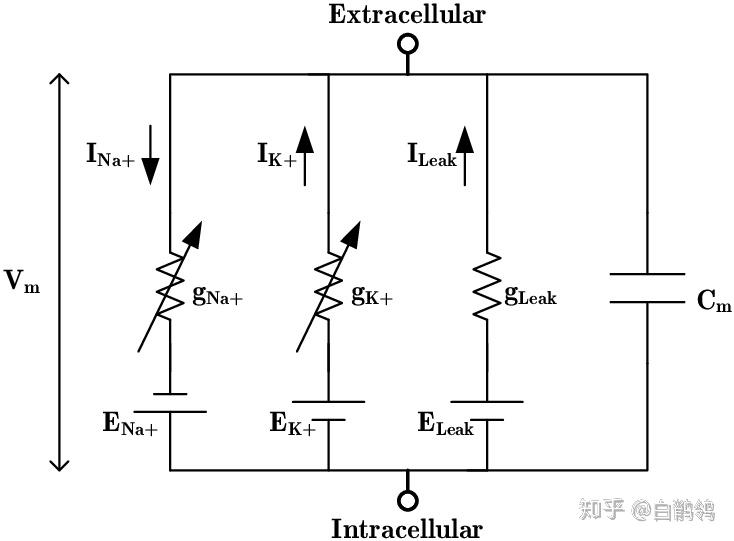
\includegraphics[width=\linewidth]{image/HH.jpg} 
  % 图片的标题在下方,是正确的
  \caption{图片来自\href{https://pica.zhimg.com/v2-7fb5b005d30ef4b685eda0643fea9270_1440w.jpg}{知乎}}
  \label{HH}
\end{marginfigure}

模型核心方程如下所示

\begin{align}
C_m \frac{dV}{dt} &= I_{\text{syn}} - \left( I_{\text{Na}} + I_{\text{K}} + I_{\text{L}} \right), \\
I_{\text{Na}} &= \bar{g}_{\text{Na}} m^3 h \left(V - E_{\text{Na}}\right), \\
I_{\text{K}}  &= \bar{g}_{\text{K}} n^4 \left(V - E_{\text{K}}\right), \\
I_{\text{L}}  &= \bar{g}_{\text{L}} \left(V - E_{\text{L}}\right),
\end{align}
相关参数更新方程可以表示成下面的方程,其中$\alpha \ \beta$都随膜电位的变化而变化
\begin{align}
\frac{dm}{dt} &= \alpha_m(V)(1-m) - \beta_m(V)m, \\
\frac{dh}{dt} &= \alpha_h(V)(1-h) - \beta_h(V)h, \\
\frac{dn}{dt} &= \alpha_n(V)(1-n) - \beta_n(V)n.
\end{align}

\subsection{无外电流刺激时}
在没有电流刺激时,膜电位倾向于进入稳态(在系统参数固定时稳态具有唯一性),此时平衡点方程为
\[
\frac{dV}{dt} = \frac{dm}{dt} = \frac{dh}{dt} = \frac{dn}{dt} = 0 
\]
即可以得到参数m、n、h的最终稳态条件为如下所示方程组
\[
m_v = \frac{\alpha_m}{\alpha_m + \beta_m}, \ n_v = \frac{\alpha_n}{\alpha_n + \beta_n}, \ h_v = \frac{\alpha_h}{\alpha_h + \beta_h}
\]
通过求解上述关于V的方程组即可解得唯一稳态电压V(在代码初始条件下达到稳态时V $\approx$ 65),即是增大或者减小初始电压值也不会影响最终稳态的大小

\begin{figure}[htbp]
    \centering
    \begin{subfigure}[t]{0.32\linewidth}
        \centering
        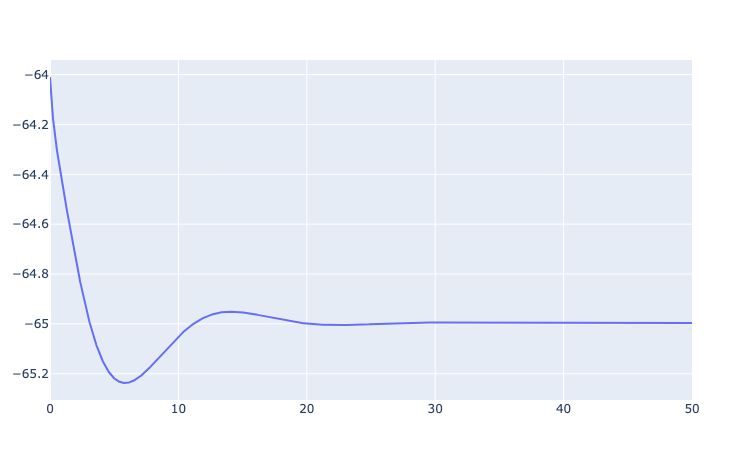
\includegraphics[width=\linewidth]{image/v64.png}
        \caption{V = 64}
        \label{fig:sub1}
    \end{subfigure}
    \hfill
    \begin{subfigure}[t]{0.32\linewidth}
        \centering
        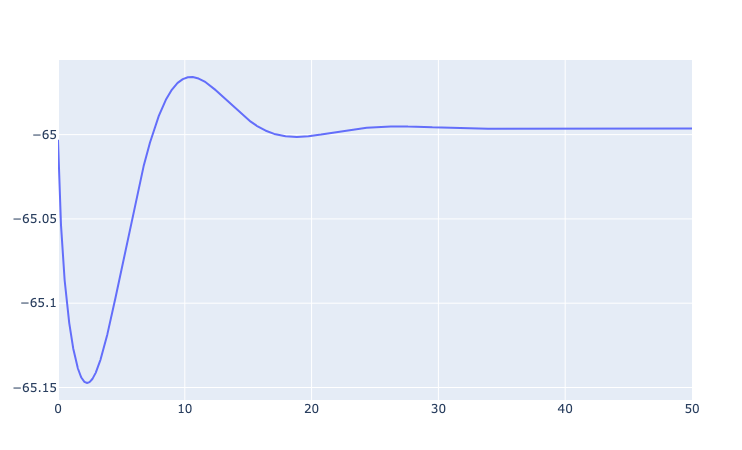
\includegraphics[width=\linewidth]{image/v65.png}
        \caption{V = 65}
        \label{fig:sub2}
    \end{subfigure}
    \hfill
    \begin{subfigure}[t]{0.32\linewidth}
        \centering
        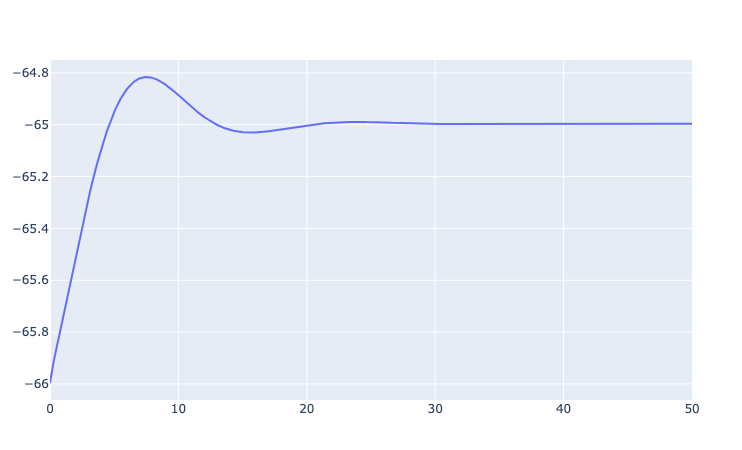
\includegraphics[width=\linewidth]{image/v66.png}
        \caption{V = 66}
        \label{fig:sub3}
    \end{subfigure}
    \caption{V初始值不同的情况下的电位变化情况,可以看出虽然变化曲线不同但是最终稳态数值都是在65mV}
    \label{fig:all}
\end{figure}

可以在运行结束达到稳态后查看m、n、h的值看是否符合上述假设
\begin{lstlisting}
  print(m,h,n)
  # m = 0.052955138647434404
  # h = 0.5960105170018434
  # n = 0.3177330523286259
\end{lstlisting}
(当我们把m、h、n的初始值设置为稳态时的值时可以发现膜电位曲线不再发生大幅度波动,而是稳定在64.996mv左右)

\subsection{给予电流刺激时}
\paragraph{施加微小刺激}
当受到外界刺激时,部分钠离子的通道会迅速地打开一段时间然后逐渐关闭,而钾离子的通道则需要一定的时间缓缓开放,因此当刺激不大时,先开启的那部分钠离子通道使得大量钠离子内流、膜电位升高,之后开启的钾离子通道则使钾离子流向细胞外、膜电位重新降低

\paragraph{施加较大刺激}
当外界刺激增大到一定程度时,由于膜电位的大幅变化使得更多电压控制的钠离子通道打开,更多的钠离子内流,大量内流的钠离子使得膜电位迅速升高至0以上产生动作电位。
而在电压升高后,并不会直接达到钠离子平衡电压,此时钠离子通道开始失活同时钾离子通道开始,两者共同作用下膜电位开始下降。而由于钠离子通道的大量失活且钾离子通道关闭的速率较慢,
细胞膜电位在之后的一小段时间甚至会降到惊喜电位以下(也被称为超极化)。此时细胞膜进入一小段不应期,之后便重新回到静息电位并且等待下一次刺激的到来。

\begin{figure*}[htbp]
    \centering
    \begin{subfigure}[t]{0.45\linewidth}
        \centering
        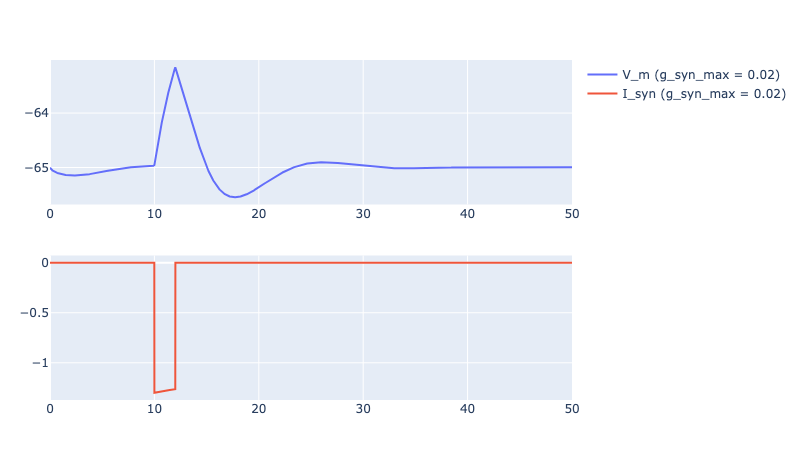
\includegraphics[width=\linewidth]{image/littleSTI.png}
        \caption{微小刺激}
    \end{subfigure}
    \hfill
    \begin{subfigure}[t]{0.45\linewidth}
        \centering
        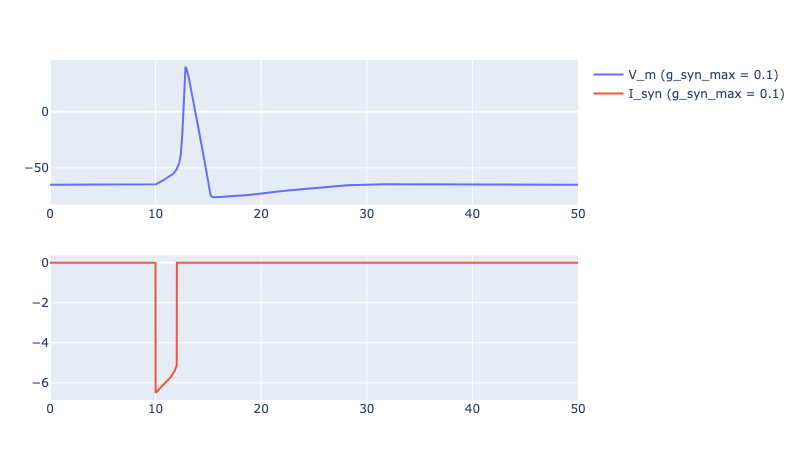
\includegraphics[width=\linewidth]{image/largeSTI.png}
        \caption{较大刺激}
    \end{subfigure}
    \caption{两种刺激下膜电位变化}
    \label{fig:input}
\end{figure*}

\paragraph{不同刺激下的膜电位变化}
刺激的大小会影响膜电位变化的幅度与速率,较小的电流刺激并不会让膜电位达到阈值而产生动作电位,较大的电流则会让膜电位升高的速率加快,从而在更短的时间内达到动作电位。
通过改变不同的输入的大小,可以绘制出在不同刺激下膜电位的变化曲线图,内容如下图所示

\begin{figure*}
  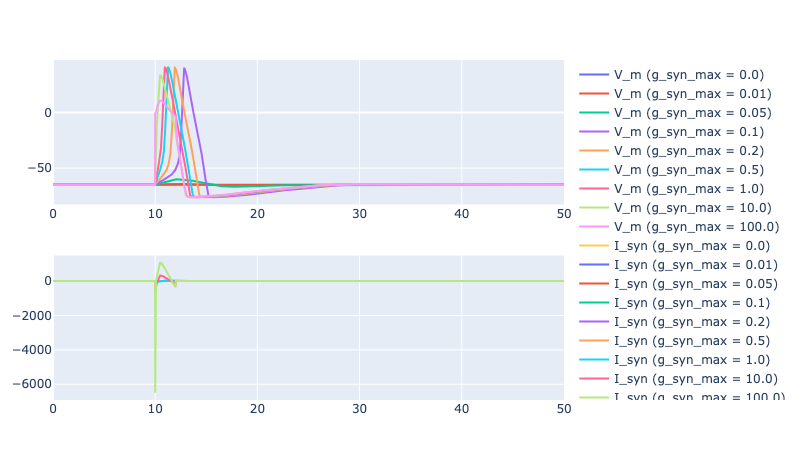
\includegraphics[width = 0.95\linewidth]{image/multople_input.png} 
  % 图片的标题在下方,是正确的
  \caption{不同输入的电位变化}
  \label{mutilple}
\end{figure*}

\section{Cable Theory}
Cable Theory是将神经细胞的突触看作一段漏电的电缆,该理论的核心可以用下面的公式来表示

\begin{marginfigure}
  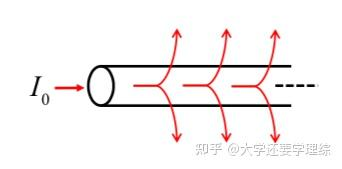
\includegraphics[width=\linewidth]{image/Cabel Theory.jpg} 
  % 图片的标题在下方,是正确的
  \caption{示意图}
  \label{Cable Theory}
\end{marginfigure}
\[
c\frac{\partial V}{\partial t} = -g_L(V - E_L) + I_{inj} + \frac{d}{4r_a}\frac{\partial^2 V}{\partial x^2}
\]

上述PDE方程主要由是三部分组成

- 扩散项:$\frac{d}{4r_a}\frac{\partial^2 V}{\partial x^2}$

- 漏电项:$-g_L(V - E_L)$

- 注入项:$I_{inj}$

实验代码中将突触建模成一个粗细均匀的电缆,且在突触中点位置注入电流,绘制出电流随着时间和空间的变化曲线图\ref{cable theory}
\begin{figure*}
  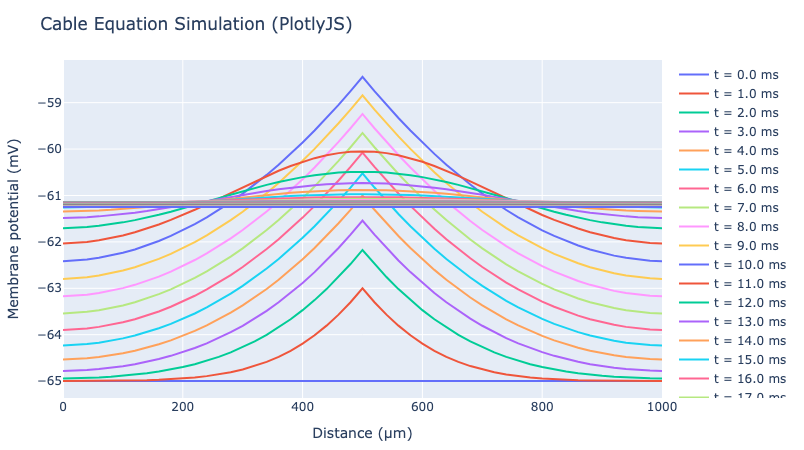
\includegraphics[width=\linewidth]{image/cable1.png} 
  % 图片的标题在下方,是正确的
  \caption{cable theory 1}
  \label{cable theory}
\end{figure*}

从图像中可以看出,初始时稳态电压在-65ms,这是因为初始时没有外部电流注入,从PDE方程中可以看出稳态条件为$0 = -g_L (V - E_L)$,即$V = E_L = -65ms$

而在之后有稳定电流注入后稳态方程则需要满足$V = E_L + \frac{I_{inj}}{g_L}$,所以在图中当t越来越大时,膜电位从之前的-65ms逐渐变成了-61.14ms(即在有恒定电流输入后的平衡膜电位)

此外,因为上述cable方程中并没有限制电流影响传播的速度,所以在这个假设下所有位置都是同时收到电流刺激的影响,在绘制不同位置随时间变化曲线时可以看出所有位置的电位都是同时产生了变化,在刺激停止后也几乎是同时衰减结束
\begin{figure*}
  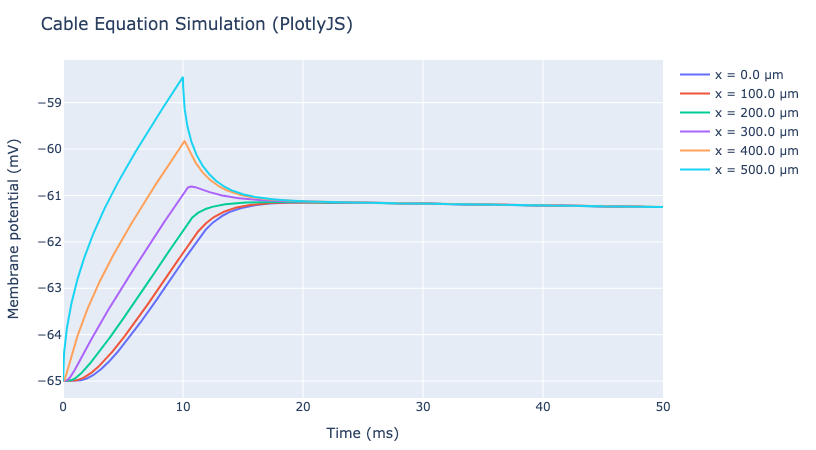
\includegraphics[width=\linewidth]{image/cable2.png} 
  % 图片的标题在下方,是正确的
  \caption{cable theory 2}
  \label{cable}
\end{figure*}

\end{document}